
\documentclass{acm_proc_article-sp}

\usepackage{amsmath}
\usepackage{verbatim}
\usepackage{textcomp}
\usepackage{graphicx}
\usepackage{subcaption}
\usepackage{url}
\usepackage{multicol}
\usepackage{tikz}
\usetikzlibrary{positioning}
\usepackage{wasysym}
\usepackage{adjustbox}
\usepackage{graphicx}
\usepackage{caption}


\begin{document}

\title{Where am I? \\ Predicting Montreal Neighbourhoods \\from Google Street View Images  \\
{\normalsize Code available at: \url{https://github.com/slflmm/Miniproject-4}}} 
\subtitle{COMP 598 -- Miniproject 4}

\numberofauthors{3} 
\author{
% 1st. author
\alignauthor 
Stephanie Laflamme\\
	\affaddr{260376691}
\alignauthor
Benedicte Leonard-Cannon\\
	\affaddr{260377592}
% 2nd. author
\alignauthor Sherry Ruan\\
	\affaddr{0000}
% 3rd. author
}

\date{Oct15}



\maketitle
\begin{abstract}
In this paper, we present a machine learning approach to classifying photographs of nine Montreal neighborhoods acquired from Google Street View. We show results using a perceptron, a stacked denoising autoencoder (to pretrain a neural network), and a convolutional neural network. We put these results in perspective by comparing them with human performance on the same task; the mean human error rate is 71.6\%. The convolutional neural network outperforms both human and other algorithmic classifiers, with an error rate of 42.61\%. We conclude by discussing the implications of our results and future avenues of research. 


\end{abstract}

\section{Introduction}% overview of approach
To a local resident, neighborhoods of the island of Montreal bear distinctive traits. For instance, Old Montreal is characterised by its historic buildings, Downtown Montreal by its skyscrapers and Westmount by its opulent houses. To the experienced human eye, it is usually possible to pinpoint the district at which a given picture was taken, granted high enough resolution. Can we say the same of machine learning algorithms?  

We attempt to determine whether machine learning algorithms can be trained to differentiate between nine visually distinctive neighbourhoods on the island of Montreal based on Google Street View images \footnote{\url{https://www.google.com/maps/views/u/0/streetview?gl=us}}. We tackle this classification problem with three models: a perceptron (as a baseline algorithm), a stacked denoising autoencoder (for neural network pretraining) and a convolutional neural network. We place the performance of these classifiers in context by comparing them with human results.

Researchers at Canergie Mellon University worked on a classification task similar to our own\cite{Doersch}. The purpose of their study was to assess how cities are uniquely defined by their visual appearance. Their approach focused on extracting unique architectural characteristics from major cities in the United States, Europe and Japan, while paying particular attention to Paris. Given labeled images acquired from Google Street View, they developed a method for automatically extracting features that are recurrent and geographically distinctive within each city. Their approach relied on discriminative clustering to extract visual cues. The researchers observed that small architectural elements such as window shapes, street signs and lamp posts tend to differentiate cities more significantly than their landmarks, such as the Eiffel tower. It is worth mentioning that this method was also applied at a smaller scale: in a vein more similar to our own prediction task, an attempt was made to distinguish between districts of Paris on the basis of architectural features.

Another similar study by Knopp et al. tackled the problem of place recognition using images of Paris acquired from Google Street View and Panoramio, a photo-sharing website \cite{Knopp}. Their objective was to automatically extract from a database a set of images representing the same location as that of a query image, regardless of the viewpoint and lighting conditions. Their place recognition algorithm used a visual bag-of-words approach combined with the filtering of confusing features such as trees or cars. 

Our research follows from these studies, albeit on a more local scale. On a broader scale, it falls under the umbrella of automatic classification of images by provenance. Success in such an endeavour would have cultural and social value; tourists could easily identify the origin of their photos, and animation studios might use these classifiers to reconstruct more vivid and evocative scenery \cite{Doersch}. Optimally, automatic place recognition could help in investigations where photographs of unidentified locations might prove crucial. 


\section{Dataset}

\subsection{Description}
We consider nine of Montreal's most distinctive neighbourhoods as classes, listed in Table \ref{tbl:boroughlist}. The dataset consists of 72,000 greyscale images of size $100\times100$, with 8000 images per neighbourhood. The data is subdivided into a training set of 64,800 images and a test set with the remaining 7,200 images. 

\begin{table}[h!]
\caption{Class labels and corresponding neighborhood}
\label{tbl:boroughlist}
\centering
\begin{tabular}{| c | c |}
\hline
\textbf{Label} & \textbf{Name} \\ \hline 
0 & Downtown \\
1 & Old Montreal \\
2 & Chinatown \\
3 & Gay Village \\
4 & Plateau \\
5 & Outremont \\
6 & Westmount \\
7 & Hochelaga \\
8 & Montreal-Nord \\ \hline
\end{tabular}
\end{table}

\subsection{Acquisition}
We use the Google Street View API \footnote{\url{https://developers.google.com/maps/documentation/streetview/}} to collect images from the neighbourhoods of interest. The API allows users to download an image based on its geographical coordinates (latitude and longitude), and to define `heading' (the camera's orientation in the x-y plane), `pitch' (the camera's orientation in the z plane, relative to the ground), as well as the field of view and size of collected images. 

Data from the City of Montreal \footnote{\url{http://ville.montreal.qc.ca/portal/page?_pageid=5798,85813661&_dad=portal&_schema=PORTAL}} is used to identify the delimiting streets of our nine neighbourhoods. We then match their intersections to geographical coordinates to obtain the vertices, also in geographical coordinates, of polygons surrounding the neighbourhoods.  Since the API enables us to poll for images based on geographical coordinates and that such coordinates are known for each neighborhood, labeling the images becomes a trivial concern.

We collect 400$\times$400 images with a field of view of 100. For each image, the heading is set to a random number between 0 and 360, and the yaw is randomly selected between 0 and 35 degrees. Figure \ref{fig:sample-images} shows a sample image from each neighbourhood. When there is no Street View panorama available at a geographical coordinate, the API returns a blank image; we identify and discard them online, as images are collected.

Once collected, images are downsampled from their original size to 100$\times$100 pixels and converted to grayscale; larger datasets did not fit into GPU memory.

\begin{figure}[h!]
\centering
	\begin{subfigure}[b]{0.3\linewidth}
		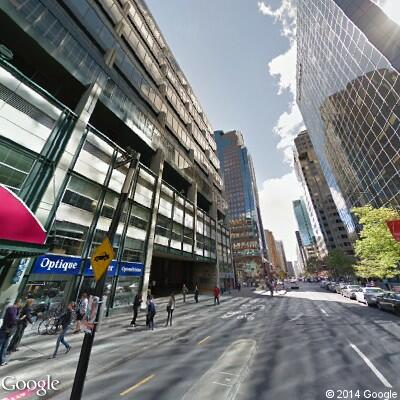
\includegraphics[width=\linewidth]{downtown.png}
		\caption{Downtown}
		\label{fig:downtown}
	\end{subfigure}
	\begin{subfigure}[b]{0.3\linewidth}
		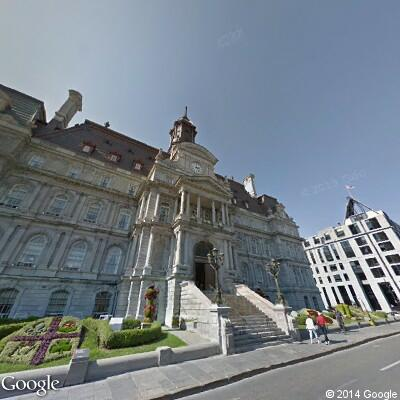
\includegraphics[width=\linewidth]{oldmontreal.png}
		\caption{Old Montreal}
		\label{fig:oldmontreal}
	\end{subfigure}
	\begin{subfigure}[b]{0.3\linewidth}
		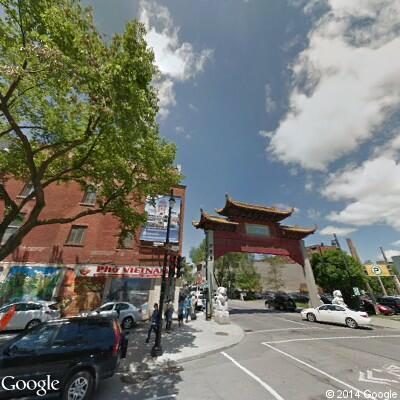
\includegraphics[width=\linewidth]{chinatown.png}
		\caption{Chinatown}
		\label{fig:chinatown}
	\end{subfigure}

	\begin{subfigure}[b]{0.3\linewidth}
		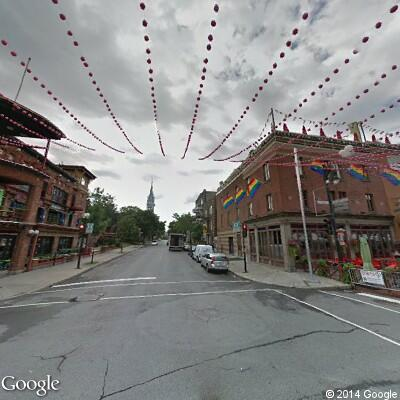
\includegraphics[width=\linewidth]{gayvillage.png}
		\caption{Gay Village}
		\label{fig:gayvillage}
	\end{subfigure}
\begin{subfigure}[b]{0.3\linewidth}
		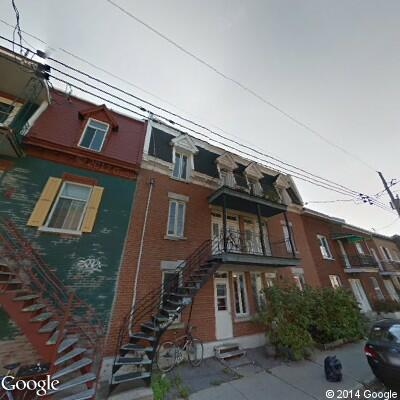
\includegraphics[width=\linewidth]{plateau.png}
		\caption{Plateau}
		\label{fig:plateau}
	\end{subfigure}
	\begin{subfigure}[b]{0.3\linewidth}
		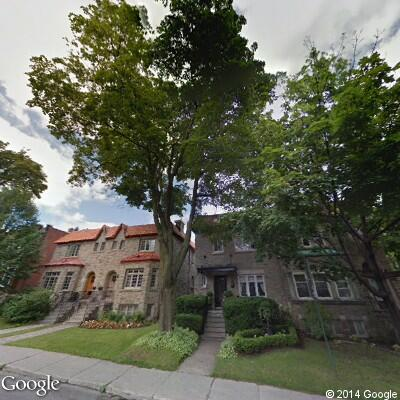
\includegraphics[width=\linewidth]{outremont.png}
		\caption{Outremont}
		\label{fig:outremont}
	\end{subfigure}

	\begin{subfigure}[b]{0.3\linewidth}
		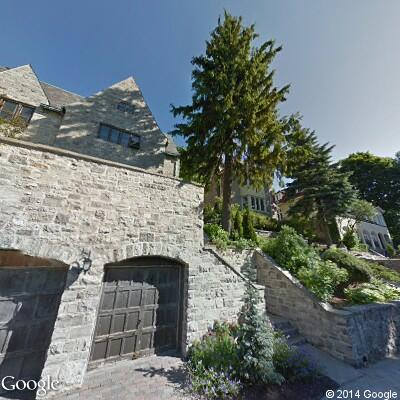
\includegraphics[width=\linewidth]{westmount.png}
		\caption{Westmount}
		\label{fig:westmount}
	\end{subfigure}
	\begin{subfigure}[b]{0.3\linewidth}
		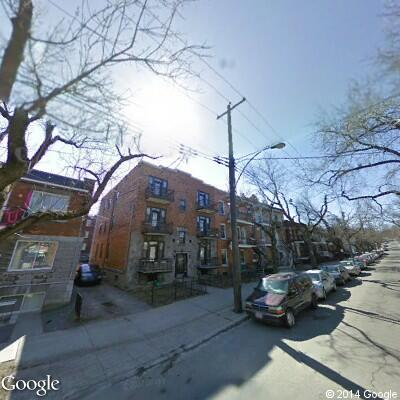
\includegraphics[width=\linewidth]{hochelaga.png}
		\caption{Hochelaga}
		\label{fig:hochelaga}
	\end{subfigure}
	\begin{subfigure}[b]{0.3\linewidth}
		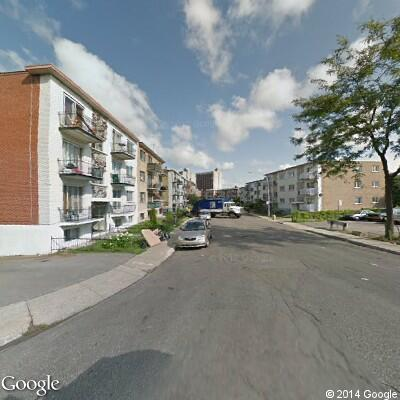
\includegraphics[width=\linewidth]{montrealnord.png}
		\caption{Montreal-Nord}
		\label{fig:montrealnord}
	\end{subfigure}
\caption{Sample images collected \label{fig:sample-images}}
\end{figure}


\subsection{Preprocessing}
As a preprocessing step, images are contrast-normalized.  Given a $100\times100$ image $x$ from the dataset, we let $$x = \cfrac{(x - x_{min})}{x_{max} - x_{min}},$$ where $x_{max}$ and $x_{min}$ are the maximum and minimum values in $x$'s pixels, respectively. This step ensures all images have the same contrast range, with pixel values ranging between 0 and 1.
\section{Classifiers}

\subsection{Human experiment}
 
To obtain a human performance baseline in comparison to machine learning methods, we conduct a small scale experiment with human participants. Five people who are familiar with the Montreal area are asked to label 50 test images of the same format as those used by our classifiers ($100\times100$ pixels, grayscale and contrast normalized). Their predictions are combined to get human labels for 250 images.

\subsection{Perceptron}
The perceptron arose from attempts at creating a machine that could recognize images \cite{Bishop}.  Inspired from neuroscience, the perceptron is made up of a single layer of `neurons'; a neuron outputs the weighted sum of all its inputs, passed through an activation function (in our case, the Heaviside step function) which ensures its output is binary. As a result, the perceptron can only learn linearly separable patterns; it cannot, for instance, encode the XOR function (which would require one more layer of neurons). As such, we implement a multiclass perceptron as a baseline classifier.

Given $n$ examples with $m$ features each, and given $k$ classes, the perceptron learns a matrix $W$ of $(m+1) \times k$ weights (one weight for each feature-class combination, and a bias vector). The perceptron is trained by gradient descent to minimize the error $$Err(x) = (y - f(W^Tx)),$$
where $f$ is the Heaviside step function, $x$ is an example, and $y$ is its class.

\subsection{Stacked denoising autoencoder} 

We evaluate the performance of a Theano-based stacked denoising autoencoder (SDA) implementation on our dataset \footnote{\url{http://deeplearning.net/tutorial/SdA.html}}. Stacked denoising autoencoders have shown to provide significant gains in accuracy at certain image classification tasks over other models such as SVMs and DBNs \cite{vincent2010}. We use Theano\cite{Theano}, a symbolic Python library that compiles computation heavy functions in C and can execute them more efficiently on a GPU. 

An autoencoder is a feedforward neural network that is given a specific objective function; find the parameter weights $W$ that can represent the input $\mathbf{x}$ at the hidden layer and reconstruct it at the output layer \cite{larochelle}. We are interested in the contents of the hidden layer once the network has been trained. The vector learned at the hidden layer vary depending on the amount of neurons it contains relative to the input layer; with fewer neurons (undercomplete representation), the hidden layer compresses the input and with more neurons (overcomplete representation), it extracts relevant features.

To find the hidden representation, $\mathbf{h}(\mathbf{x})$, and the output $\mathbf{\hat{x}}$, we perform forward propagation much like in a standard neural network. Forward propagation can be divided into two components: an encoding step,
$$h(\mathbf{x}) = sigmoid(\mathbf{b} + W\mathbf{x} ) $$
where we transform the input into its hidden representation and a decoding step,
$$\mathbf{\hat{x}} = sigmoid(\mathbf{c} + W^*\mathbf{h}(\mathbf{x}) ) $$
where we restore the input from this same latent representation \cite{larochelle}. We often rely on tied weights, meaning that the same weight matrix is used at both layers: $W^*$ corresponds to $W^T$.

The training objective of the autoencoder is to minimize the difference between the input $\mathbf{x}$ and the output $\mathbf{\hat{x}}$. In order to do so, an option is to minimize the cross entropy loss between the two,
$$l(\mathbf{\hat{x}}) = -\sum_k{x_k \log{\hat{x}_k} + (1-x_k)\log{(1-\hat{x}_k})} $$
To optimize the values for $W$, $\mathbf{c}$ and $\mathbf{ b}$ we compute their gradients and backpropagate them by gradient descent.

In our implementation, we use a denoising autoencoder. Simply put, the denoising process consists of setting some of the elements of the input $\mathbf{x}$ to $0$ with probability $p$  \cite{vincent2008}. We can achieve this by applying a Bernoulli mask to the input. We train the network by performing forward and backward propagation normally. Interestingly, denoising autoencoders tend to generate a better latent representation since they are more robust to ``partial destruction of the input'' \cite{vincent2008}. 

Classification cannot be performed with a denoising autoencoder alone. A common technique consists of stacking pretrained hidden layers of denoising autoencoders in order to build a traditional neural network. More precisely, we train an autoencoder, then connect its hidden layer to the input of the next one and so on. We train each autoencoder sequentially from the bottom up, while keeping the parameters of the previous ones fixed. Once pretraining is complete, we add an output layer to the model and we finetune this newly formed neural network using `standard' gradient descent. By pretraining a neural network in such a way, we improve its capability to generalize since the parameters are initialized to values that are closer to the global optimum than randomly initialized ones \cite{vincent2010}. 

\subsection{Convolutional neural network}

Although fully-connected stacked autoencoders tend to perform very well at machine learning tasks, their ability to classify images is sensitive to position, size, and distortions--they can be poor at identifying invariant patterns. In the early `80s, Fukushima introduced convolution layers to remedy that problem by handling geometrical similarities regardless of position \cite{Fukushima}. A convolution applies a filter $F$ to an image $X$ as follows 
$$ (X * F)_{ij} = \sum_{pq}{X_{i+p,j+q}F_{r-p,r-q}} $$
where $i,j$ are pixel indexes in the outputted convolution, $r$ is the dimension of the filter and and $p,q$ are offsets ranging from $0$ to $r-1$ \cite{larochelle_convnet}. A convolution layer contains many such filters, whose values are learned as the neural network is trained. A convolution layer thus serves as an implicit feature extractor, and is optionally followed by a pooling layer which shrinks the image by some factor. Hidden layers sit on top of a sequence of alternating convolution and pooling layers.

Our convolutional neural network uses rectifier linear units (ReLUs) as activations, written  $$f(x) = \max(0.0, x).$$ This activation function is known to perform better than bounded activations (e.g. $\tanh$) in deep neural nets for image-related tasks, presumably because they preserve intensity information about incoming information \cite{Nair}.

We also handle the overfitting that tends to happen in neural networks with many layers; there may be many complicated relationships between examples and their labels, and enough hidden units to model these relationships in multiple ways. Hinton et al. \cite{Hinton} introduced the concept of dropout to alleviate this issue. During training, hidden units are randomly omitted with probability $p$, which helps prevent complex co-adaptations on training data. We apply dropout to our convolutional neural network as Krizhevsky et al. \cite{Krizhevsky} did--that is, the fully-connected hidden layers are subject to dropout.

As convolutional neural networks tend to outperform other methods at image classification, we implement our own convolutional neural network and train it using minibatch gradient descent. Our implementation is optimized for time-efficiency and for maximizing accuracy and reducing overfitting.

Given the vast amount of time required to train a convolutional neural network, we implement ours to run on a GPU using Theano. This reduces the training time by approximately a factor of 10. To further improve performance, we use the cuda-convnet implementation of convolutions \cite{Krizhevsky}, which offers a 3-fold speed improvement relative to Theano's convolution function.

\section{Hyperparameter Selection}

\subsection{Perceptron}

Using a cross-validation procedure with the training set, we perform gridsearch over two parameters; the learning rate and the number of training iterations. We consider values between 0.0001 and 0.1 for the learning rate $\alpha$, and values between 10 and 35 for the number of iterations. We record the validation and training errors for each hyperparameter combination. We then use our best parameter settings according to the validation error to train the perceptron on the whole training set, and measure its error on the test set.

\subsection{Stacked denoising autoencoder}

We greedily search over several parameters: the pretraining learning rate, the number of pretraining epochs, the finetuning learning rate, the hidden layer count and sizes, the level of noise in each layer, and the L1 and L2 regularization coefficients. For each parameter setting, the network is trained for 120 epochs. We record the best validation error obtained, as well as the training error achieved at the same epoch. Finally, we save the predictions of our best model and compute its error against the test set.

\subsection{Convolutional network}
As we do for the stacked autoencoder, we perform greedy search over the space of hyperparameters. We consider as parameters the learning rate, the number of convolutional layers, the sizes of filters in each layer, the amount of downsampling applied after each layer, the number of hidden layers, the number of hidden units per hidden layer, and the number of training epochs. For each hyperparameter setting, we keep track of the best validation error and its corresponding training error. Once again, we save the test set predictions of our best model to calculate the testing error.

\section{Results}
We report results for our three classifiers and human labeling. In general, convolutional neural networks outperform the stacked autoencoders, which in turn exceeds the baseline results from the perceptron.

\subsection{Human experiment}

Human labelers had error rates ranging from 66\% to 80\%, with a mean of 71.6\% error. Figure \ref{fig:human-conf} shows the confusion matrix of their combined predictions. Generally, humans are good at identifying images from the Downtown neighbourhood, as well as those from Westmount. Moreover, they succeed at separating residential areas from commercial areas; they tend to confuse the residential neighbourhoods with each other (Westmount, Outremont, Montreal-Nord, Hochelaga), and predict images from more touristy areas (Downtown, Chinatown, Gay Village, Old Montreal) as being taken in the Downtown area.

\begin{figure}[h!]
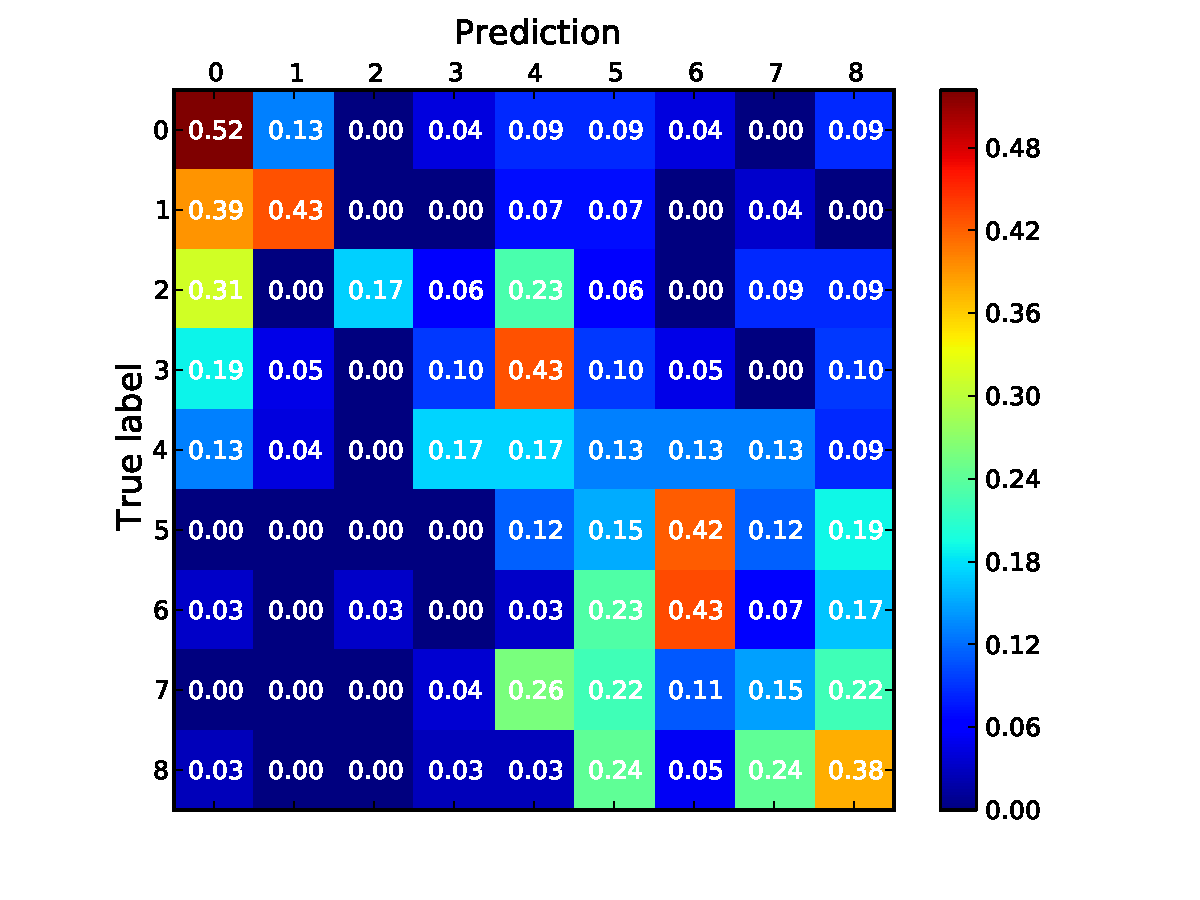
\includegraphics[width=\linewidth]{human_confusion.pdf}
		\caption{Confusion matrix for human labelers}
		\label{fig:human-conf}
\end{figure}

\subsection{Perceptron}

The cross-validation procedure for the perceptron yielded validation accuracies hovering between 12-14\%. Figure \ref{fig:perceptron-crossval} shows the effects of varying the learning rate $\alpha$ and number of training iterations on cross-validation accuracy; the optimal configuration achieved 13.99\% accuracy, with $\alpha = 0.001$ over 35 iterations. 
\begin{figure}[h!]
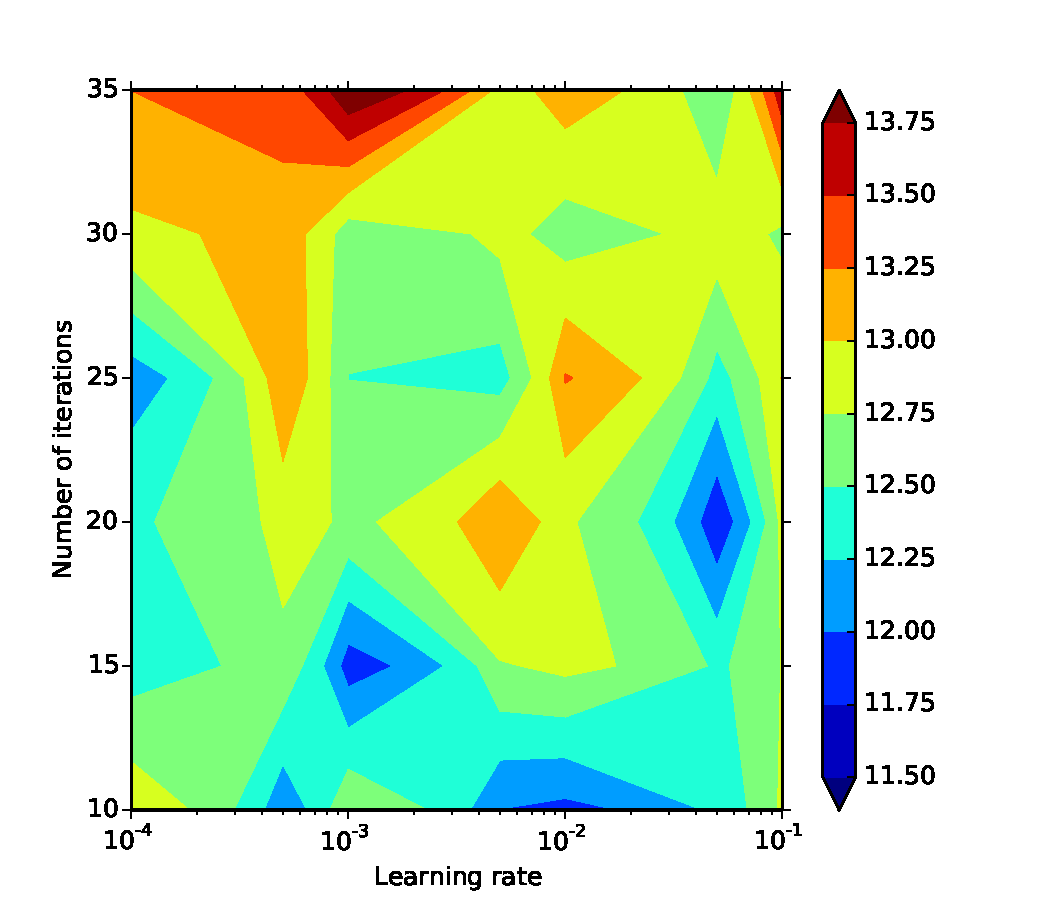
\includegraphics[width=\linewidth]{perceptron_crossval.pdf}
		\caption{Cross-validation results for the perceptron}
		\label{fig:perceptron-crossval}
\end{figure}

Training with these optimal hyperparameters led to an accuracy of 13.88\% on the test set, a result which is only slightly better than a random classifier (which has an accuracy of $1/9 = 11.\bar{11}$). Figure \ref{fig:perceptron-conf} shows the confusion matrix over the test set. Interestingly, it seems that the perceptron obtained slightly better-than-random results by simply over-predicting three classes (Downtown, Outremont, and Montreal-Nord). 
\begin{figure}[h!]
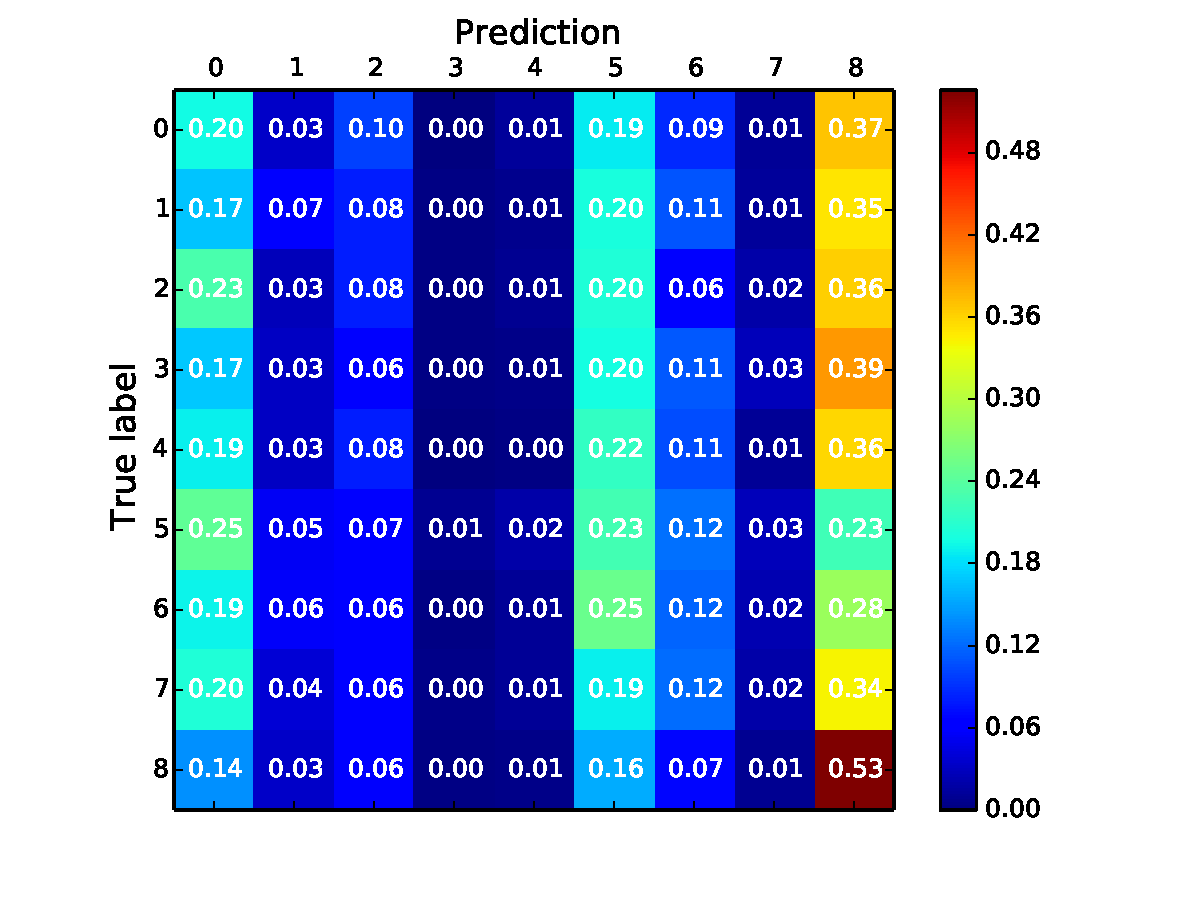
\includegraphics[width=\linewidth]{perceptron_confusion.pdf}
		\caption{Confusion matrix for the perceptron}
		\label{fig:perceptron-conf}
\end{figure}


\subsection{Stacked denoising autoencoder}

We performed validation experiments over a set of hyperparameters outlined in Table \ref{tab:sda_params} in the Appendix. Figure \ref{fig:autoencoder_compare} empirically illustrates the results of these experiments. In general, the validation error decreases steadily until epoch 40, at which point it oscillates between values of 0.75 and 0.65. Notably, the validation error during experiment 9 fluctuates more than for other experiments; this may be due to its much larger number of hidden units per layer. Indeed, while other classifiers had 500 hidden units per layer, this one boasted 1500. 

\begin{figure}[h!]
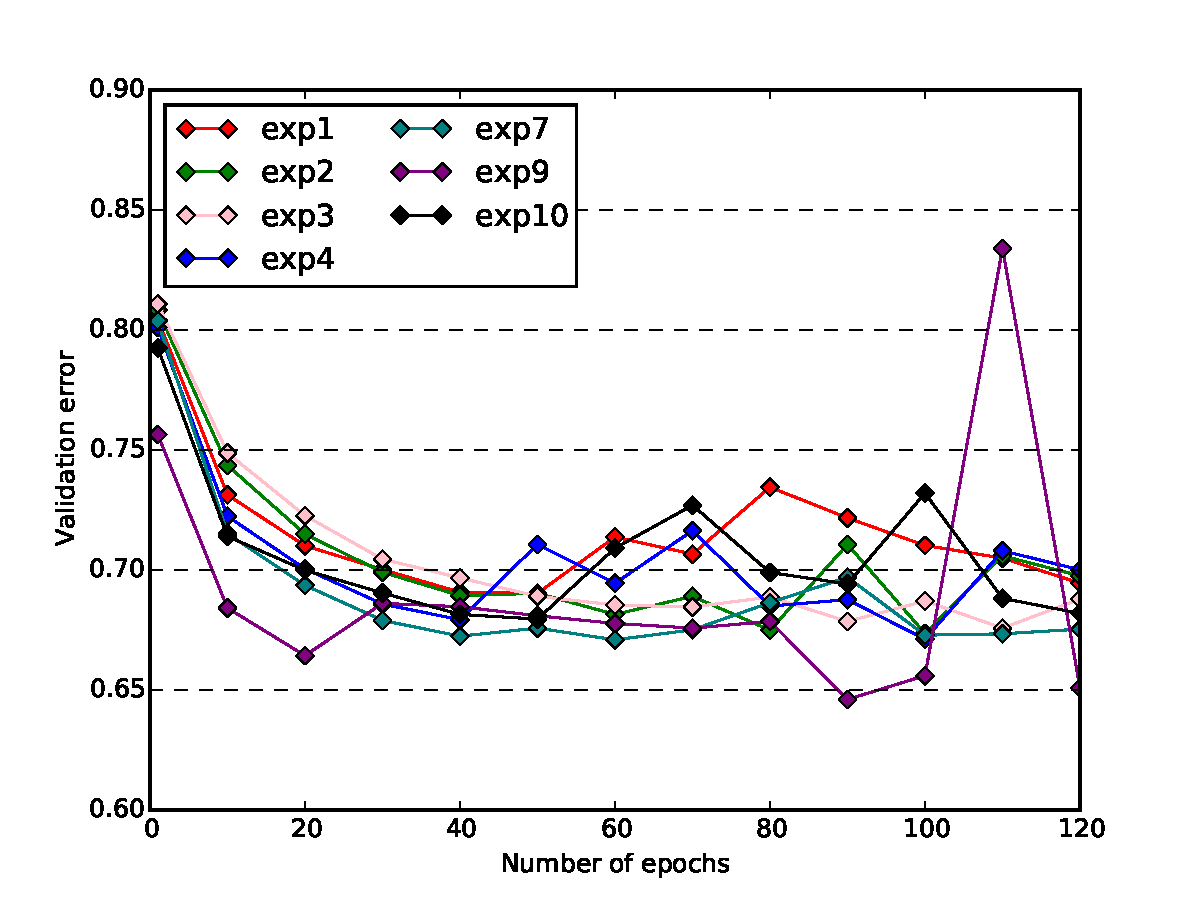
\includegraphics[width=\linewidth]{autoencoder_compare.pdf}
		\caption{Validation error of stacked autoencoder experiments}
		\label{fig:autoencoder_compare}
\end{figure}

Nonetheless, the hyperparameters used in experiment 9 produced our best validation results for the stacked denoising autoencoder, with a validation error of 64.61\%. Figure \ref{fig:autoencoder_trainvsvalid} shows a comparison of its training error and validation error over the first 120 epochs. Note that while the validation error plateaus at a high value, the training error continues to decrease steadily toward 0; it is clear that this classifier overfits.

\begin{figure}[h!]
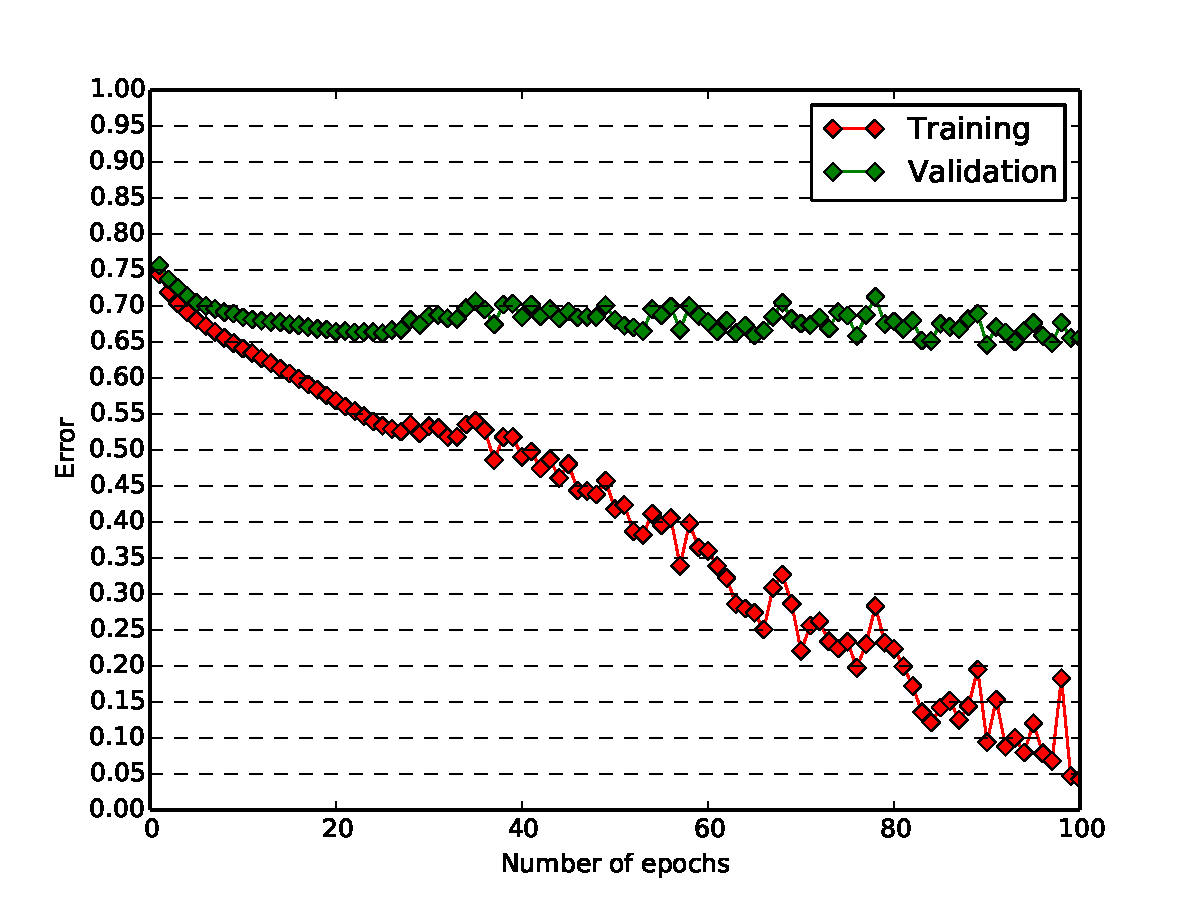
\includegraphics[width=\linewidth]{autoencoder_learning.pdf}
		\caption{Training error vs validation error for the autoencoder}
		\label{fig:autoencoder_trainvsvalid}
\end{figure}

Our best stacked denoising autoencoder gave 66.09\% error on the test set. As can be seen from the confusion matrix in Figure \ref{fig:autoencoder_conf}, the autoencoder does moderately well at identifying images from Chinatown, Old Montreal, Gay Village, Outremont, and Montreal-Nord, but is very poor at classifying images from the other neighbourhoods, especially those from the Plateau.

\begin{figure}[h!]
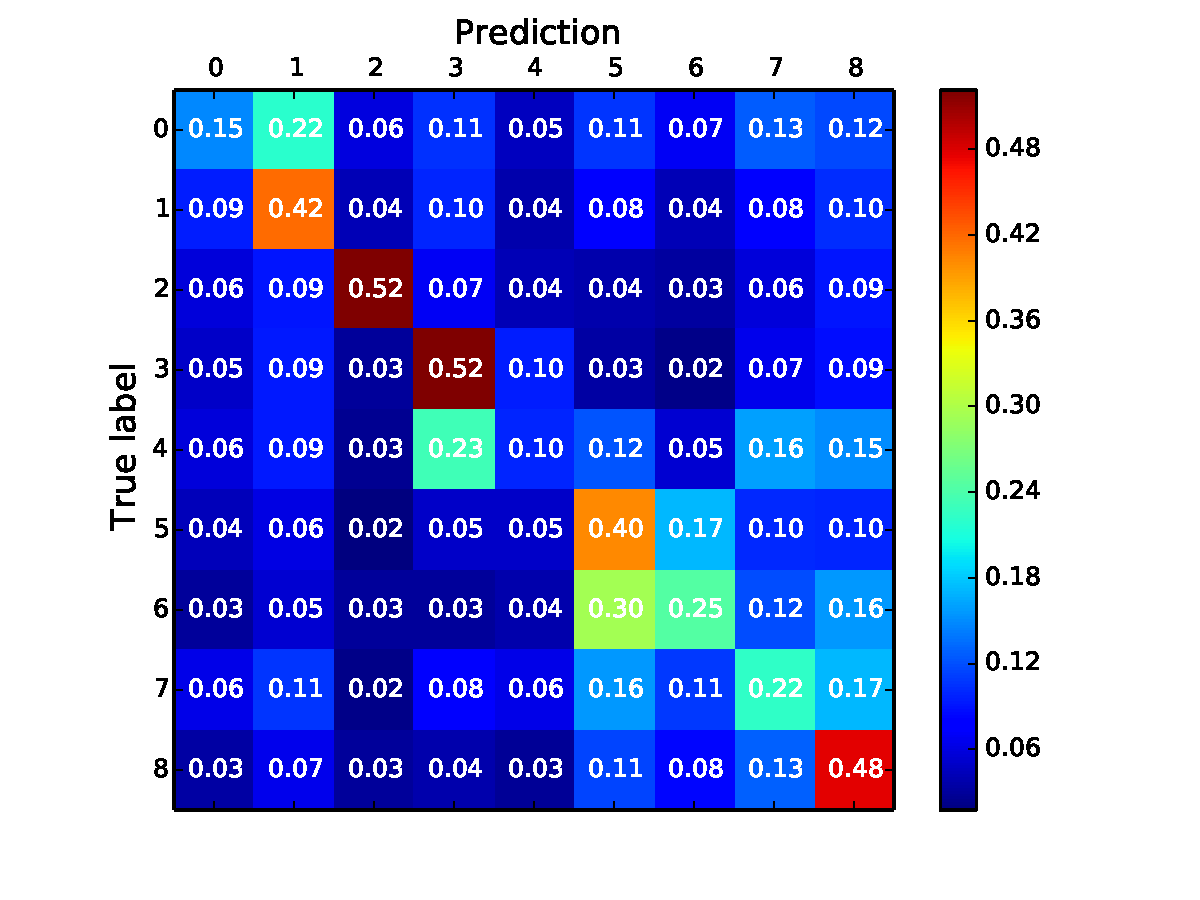
\includegraphics[width=\linewidth]{autoencoder_confusion.pdf}
		\caption{Confusion matrix for stacked denoising autoencoder}
		\label{fig:autoencoder_conf}
\end{figure}

\subsection{Convolutional neural network}

Table \ref{tab:convnet_params} in the Appendix lists the validation experiments performed with a convolutional neural network, with their hyperparameter settings and validation errors. Figure \ref{fig:convnet_compare} shows results from a subset of those experiments; observe that experiments seem to reach the beginning of a plateau by epoch 80. 

\begin{figure}[h!]
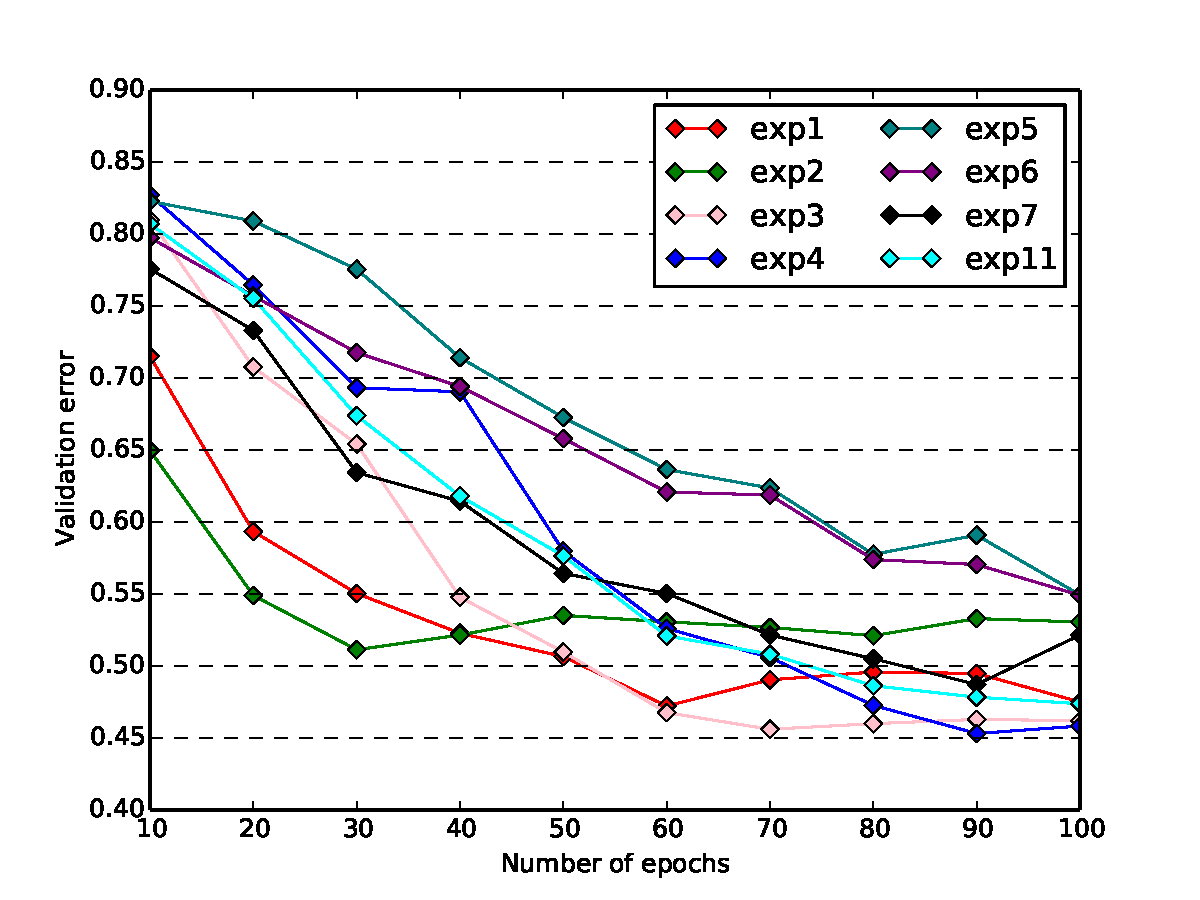
\includegraphics[width=\linewidth]{convnet_compare.pdf}
		\caption{Validation errors of convolutional neural network experiments}
		\label{fig:convnet_compare}
\end{figure}

Our best validation results were obtained in experiment 4, with a validation error of 42.82\% after 200 epochs. Figure \ref{fig:convnet_trainvsvalid} shows a comparison of the validation error versus the training error over time. One can see that the validation error reaches a plateau while the training error continues to decrease; the convolutional neural network overfits somewhat, but not so dramatically as the stacked denoising autoencoder.

\begin{figure}[h!]
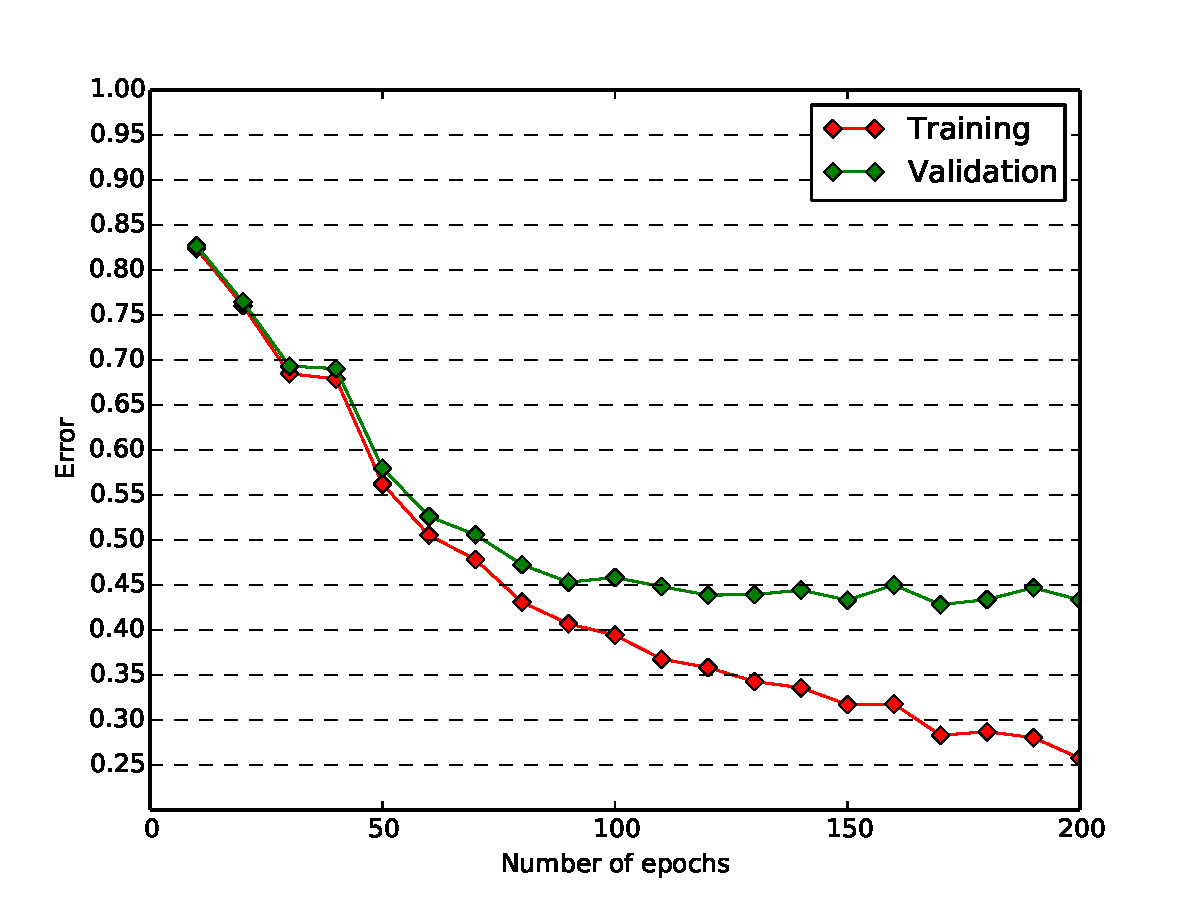
\includegraphics[width=\linewidth]{convnet_learning.pdf}
		\caption{Training error vs validation error for the convolutional neural network}
		\label{fig:convnet_trainvsvalid}
\end{figure}

Our best convolutional neural network obtained 42.61\% testing error. The confusion matrix, shown in \ref{fig:convnet_confusion} demonstrates that the classifier is best at identifying images from Chinatown and the Gay Village. On the other hand, it completely fails to correctly classify images taken in the Plateau, misclassifying them as taken in the Gay Village. The classifier shows a moderately good performance for the other neighbourhoods.

\begin{figure}[h!]
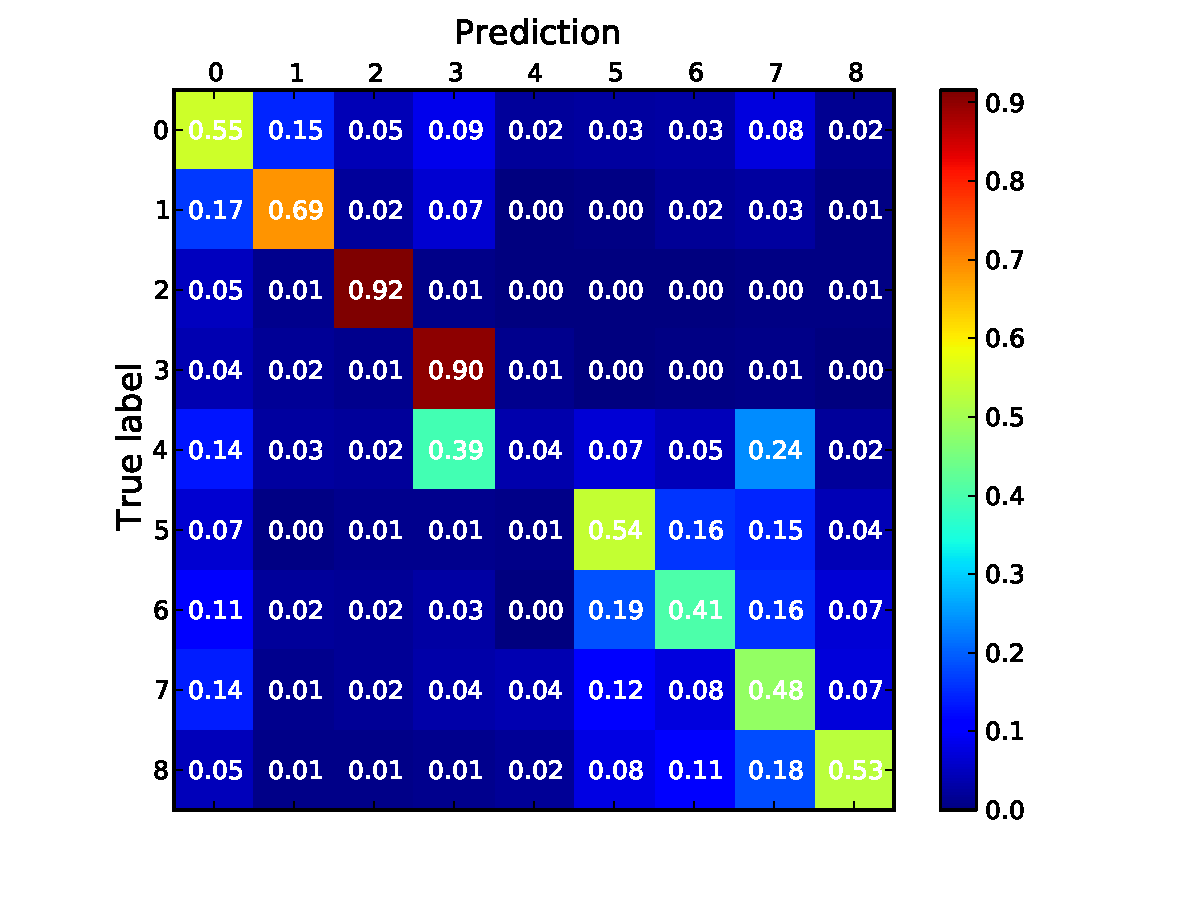
\includegraphics[width=\linewidth]{convnet_confusion.pdf}
		\caption{Confusion matrix for the convolutional neural network}
		\label{fig:convnet_confusion}
\end{figure}

\section{Discussion}% pros/cons of approach & methodology (and alternatives)
We have seen results from three machine learning classifiers. The perceptron only performed slightly better than random by over-predicting three labels. It was outmatched by the stacked denoising autoencoder, which obtained 66.09\% error--a result slightly better than human performance, which achieved 71.6\% error. However, the convolutional neural network did better by far than any of our other classifiers, with 42.82\% error. 

It is interesting to note the differences between humans and machine learning algorithms in terms of their patterns of inaccuracy. Indeed, while humans tended to have confusion between all residential areas, the convolutional neural network and stacked autoencoder were able to distinguish between them much more reliably.  Moreover, while both humans and classifiers had difficulty with correctly labeling images from the Plateau, they show very different responses. The machine learning classifiers tended to simply predict most Plateau images as being from the Gay Village or Hochelaga, whereas humans had a more spread out guessing pattern. Finally, whereas algorithms were very good at labeling images from Chinatown and the Gay Village, humans tended to think they were from Downtown or the Plateau; in general, humans overpredicted neighbourhoods near the Downtown area as being from Downtown. It is worth mentioning that the poor accuracy of human labelers who, however, were familiar with Montreal neighborhoods, can be explained by the poor image resolution. We extrapolate that humans would perform better with bigger images.

We expect that the poor performance of both humans and learning algorithms when it comes to labeling images from the Plateau can be attributed to attributes of the Plateau itself. Indeed, it may look too similar to other neighbourhoods to be reliably identified from images; as a result, humans confound it with other labels, and classifiers rarely predicted Plateau as a label. 

As for the disproportionate success of learning algorithms in identifying images from Chinatown and the Gay Village, we posit that the small size of these neighbourhoods was responsible. Since we collected the same number of images from each of the nine neighbourhoods, it is inevitable that there will be more redundancy in smaller neighbourhoods than in larger ones; for instance, the same building, seen from different angles, is likely to appear multiple times in the former. New examples may frequently look very similar to some training example, making it easier to classify.

The convolutional neural network has as its strong point the ability to learn scale- and location-invariant features in its filters. We can see from Figure \ref{fig:convnet_filters}, which shows the filters of the first convolutional layer, that the network learns a variety of edge and corner detectors, as well as an assortment of other patterns. We believe that the visual patterns learned by the convolutional neural network's filters are behind its superior performance  compared to the stacked denoising autoencoder.

\begin{figure}[h!]
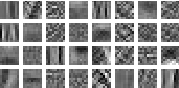
\includegraphics[width=\linewidth]{convnet_filters.pdf}
		\caption{First-layer filters from the convolutional neural network}
		\label{fig:convnet_filters}
\end{figure}

It should also be noted that the results we obtained using the convolutional neural network are unlikely to be the best we could have obtained. Indeed, we were limited by our GPU's memory capacity. We could fit neither larger images (either in terms of pixel size or colour) nor larger neural networks into its memory.

Our results can therefore only serve as a preliminary evaluation of the task's difficulty; we have seen that machine learning methods can outperform humans familiar with the task domain, but can only produce a lower bound on accuracy.

\subsection{Future work}
New avenues could be explored in order to obtain better accuracies. There are two routes to take; the first focuses on enriching our dataset, while the second emphasizes algorithmic techniques. 

Improvements to the dataset may well yield an increased accuracy. One option is to capture Street View images that are strictly parallel to their streets of origin (rather than at random angles), in order to collect more images of facades and fewer images of streets. We believe that the former are more discriminant than the latter, since roads tend to look alike across all classes. Another means of enriching our dataset consists of using larger images in colour, with the drawback of requiring more computing resources (e.g. extra GPUs and computation time).  We might also improve our results taking a set of $n$ sub-images and their horizontal reflections for each image, and combining these elements to form our dataset; this technique reduced overfitting with the ImageNet dataset\cite{Krizhevsky}. Finally, with classifiers other than the convolutional neural network, we might take an approach similar to Knopp's\cite{Knopp}, and featurize our dataset using the visual-bag-of-words technique, removing confusing features that tend to be present in images of all classes--such as cars and people.

There are also improvements to be made from an algorithmic point of view. We can focus on improving our best classifier--the convolutional network. Conducting a more thorough parameter search, for instance with the Spearmint library \footnote{\url{https://github.com/JasperSnoek/spearmint}} for Bayesian optimization might lead to significant gains in performance. Moreover, we might introduce momentum to our weight updates; it allows for an update proportional to previous updates--yielding bigger updates when the gradient's direction remains unchanged, and slowing the updates when it varies. This approach is helpful in avoiding local optima\cite{sutskever}. 

In this paper, we presented a machine learning approach to automatic provenance recognition of images from neighbourhoods on the island of Montreal. The convolutional neural network model led to promising preliminary results. Given the richness of possible improvements over our work, we hope to motivate further research in the same vein. 

{\bfseries We hereby state that all the work presented in this report is that of the authors.}

\bibliographystyle{abbrv}
\bibliography{references}

\newpage

\appendix
\label{appendix}
\begin{table*}
\caption{Average training and validation errors based on hyperparameter configuration for the stacked denoising autoencoder}
\label{tab:sda_params}
\begin{center}
\begin{adjustbox}{width=\textwidth}
\begin{tabular}{lccccccccc|rr|}

{\bf Experiment} & {\bf Pretrain lr} & {\bf \# Pretrain epochs}
&{\bf Finetune lr}
&{\bf \# Train epochs}
&{\bf \# Hidden layers}
&{\bf Layer noise}
&{\bf L1 factor}
&{\bf L2 factor}
&{\bf Error (train)}
&{\bf Error (valid.)}
\\ \hline \\	
1 & 0.001 & 20 & 0.1 & 120 & 500, 500 & 0.1, 0.2 & 0 & 0 & 0.59727431 & 0.68889509 \\
2 & 0.001 & 20 & 0.1 & 120 & 500, 500, 500 & 0.1, 0.2, 0.3 & 0 & 0 & 0.51444444 & 0.66782924 \\
3 & 0.001 & 20 & 0.1 & 120 & 500, 500, 500 & 0.2, 0.3, 0.4 & 0 & 0 & 0.48682292 & 0.67327009 \\
4& 0.001 & 20 & 0.2 & 120 & 500, 500, 500 & 0.1, 0.2, 0.3 & 0 & 0 & 0.33623264 & 0.67117746 \\
5 & 0.001 & 20 & 0.2 & 120 & 500, 500, 500 & 0.3, 0.4, 0.5 & 0 & 0 & 0.28029514 & 0.68317522 \\
6 & 0.001 & 20 & 0.2 & 120 & 250, 250, 250 & 0.1, 0.2, 0.3 & 0 & 0 & 0.58552083 & 0.69963728 \\
7 & 0.005 & 20 & 0.2 & 120 & 500, 500, 500 & 0.1, 0.2, 0.3 & 0 & 0 & 0.44685764 & 0.66266741 \\
8 & 0.005 & 20 & 0.2 & 120 & 500, 500, 500 & 0.25, 0.25, 0.25 & 0 & 0 & 0.51513889 & 0.66503906 \\
9 & 0.005 & 20 & 0.2 & 120 & 1500, 1500 & 0.25, 0.25 & 0 & 0 & 0.09411458 & 0.64606585 \\
10 & 0.005 & 20 & 0.2 & 120 & 500, 500 & 0.25, 0.25 & 1e-05 & 0 & 0.37560764 & 0.67424665 \\
11 & 0.005 & 20 & 0.2 & 120 & 500, 500 & 0.25, 0.25 & 1e-05 & 1e-05 & 0.48104167 & 0.67368862 \\
12 & 0.005 & 5 & 0.2 & 120 & 500, 500 & 0.25, 0.25 & 0 & 0 & 0.23010417 & 0.67606027 \\
13 & 0.005 & 20 & 0.2 & 120 & 500, 500 & 0.35, 0.35 & 0 & 0 & 0.54907986 & 0.67926897 \\
14 & 0.005 & 20 & 0.2 & 120 & 500, 500 & 0.35, 0.35 & 0 & 1e-04 & 0.56454861 & 0.67103795 \\
15 & 0.005 & 20 & 0.05 & 120 & 500, 500 & 0.35, 0.35 & 1e-04 & 1e-04 & 0.68671875 & 0.70438058 \\
16 & 0.001 & 5 & 0.05 & 120 & 500, 500 & 0.35, 0.35 & 1e-04 & 1e-04 & 0.72546875 & 0.74372210 \\
17 & 0.005 & 20 & 0.2 & 120 & 1500, 1500 & 0.25, 0.25 & 1e-04 & 1e-04 & 0.70560764 & 0.72154018 \\ 

\end{tabular}
\end{adjustbox}
\end{center}
\end{table*}



\begin{table*}
\caption{Average training and validation errors based on hyperparameter configuration for the convolutional neural network}
\label{tab:convnet_params}
\begin{center}
\begin{adjustbox}{width=1\textwidth}
\begin{tabular}{lcccllcc|rr}

%&\multicolumn{1}{l}{\bf Experiment}
&\multicolumn{1}{l}{\bf \# Epochs}
&\multicolumn{1}{c}{\bf Learning rate}
&\multicolumn{1}{c}{\bf Filter sizes}
&\multicolumn{1}{c}{\bf \# Filters}
&\multicolumn{1}{c}{\bf Downsampling}
&\multicolumn{1}{c}{\bf Hidden layers}
&\multicolumn{1}{r}{\bf Error (train)}
&\multicolumn{1}{r}{\bf Error (valid.)}
\\ \hline \\	
1 & 100 & 0.2 & (9, 6, 5, 5) & (32, 64, 80, 80) & (4, 2, 1, 1) & (500) & 0.353837 & 0.472238 \\
2 & 100 & 0.2 & (9, 6, 5, 5) & (32, 64, 80, 80) & (4, 2, 1, 1) & (500, 500) & 0.456059 & 0.511300 \\
3 & 100 & 0.1 & (9, 6, 5, 5) & (32, 64, 80, 80) & (4, 2, 1, 1) & (500, 500) & 0.381302 & 0.456055 \\
4 & 100 & 0.05 & (9, 6, 5, 5) & (32, 64, 80, 80) & (4, 2, 1, 1) & (500, 500) & 0.406875 & 0.453125 \\
5 & 100 & 0.025 & (9, 6, 5, 5) & (32, 64, 80, 80) & (4, 2, 1, 1) & (500, 500) & 0.430278 & 0.476283 \\
6 & 100 & 0.05 & (9, 6, 5, 5) & (32, 64, 80, 80) & (2, 2, 2, 2) & (500, 500) & 0.467639 & 0.549107 \\
7 & 100 & 0.05 & (9, 6, 5, 5) & (32, 64, 80, 80) & (4, 1, 1, 1) & (500, 500) & 0.370069 & 0.487165 \\
8 & 100 & 0.05 & (9, 6, 4, 3, 3) & (32, 64, 80, 80, 80) & (4, 2, 1, 1, 1) & (500, 500) & 0.380729 & 0.452148 \\
9 & 200 & 0.05 & (9, 6, 4, 3, 3) & (32, 64, 80, 80, 80) & (4, 2, 1, 1, 1) & (500, 500) & 0.246354 & 0.433873 \\
10 & 100 & 0.05 & (9, 6, 5, 5) & (32, 64, 80, 80) & (4, 2, 1, 1) & (500, 500) & 0.283090 & 0.428153 \\
11 & 100 & 0.05 & (9, 8, 5, 5) & (32, 64, 80, 80) & (4, 2, 1, 1) & (500, 500) & 0.392865 & 0.473772 
\end{tabular}
\end{adjustbox}
\end{center}
\end{table*}


\balancecolumns
\end{document}